\chapter{Introduction}

\section{Overview}

We propose to run human-in-the-loop subject testing experiments to understand the effects of concurrent bandwidth feedback, and to integrate the effects of this feedback into a human performance model.
To investigate the three Aims outlined in the Problem Statement, we propose two experiments and the development of a model.

\begin{description}[align=left]
    \item [Experiment One] investigates if concurrent bandwidth feedback can be used to teach novice subjects to improve performance in a three-axis manual tracking task.
    \item [Experiment Two] investigates if concurrent bandwidth feedback can decrease the required learning time to peak performance in a simulated robotic arm track and capture task.
    \item [The Model] will extend Professor Hess' structural model of the human pilot to include the effects of concurrent bandwidth feedback.
\end{description}

Concurrent bandwidth feedback has been used in a large variety of motor control tasks, and has generally been found to improve performance.
Until recently, however, only simple tasks such as physical movements or low-dimensional pursuit tasks have been investigated.
More recent works, including the lane-keeping task by de Groot et al., and our previous work with the SAFER task, have indicated that concurrent bandwidth feedback can also be quite effective for complex tasks.
Unlike simple tasks, in which the guidance hypothesis dominates when feedback is removed, there is some evidence that concurrent bandwidth feedback can be removed after training without a loss of performance.
The decrease in required learning time, improved performance, and decreased workload seen in the SAFER task show that concurrent bandwidth feedback may prove to be most useful very early in training when subjects are first exposed to complex, highly dynamic tasks.
As concurrent bandwidth feedback can improve performance without an increase in workload, it may prove a useful technique for training other robotics tasks.

There has been considerable improvement in the field of pilot modeling since McRuer's crossover model, especially with models that incorporate human physiology.
The Structural Model, in particular, has been very effective in predicting pilot performance, handling qualities, pilot-induced oscillation rating levels, and workload for a variety of system dynamics.
None of these pilot models, however, are able to include the effects of concurrent bandwidth feedback.
The performance improving effects of this feedback, seen throughout the literature, make this a compelling feature to be incorporated into a pilot model.

\subsection{Motivation}
\label{sec:intro_overview}
We aim to improve performance and decrease learning times for novice operators of highly complex motor control tasks.
We are specifically interested in modeling and improving human performance in robotic arm tasks, which generally require extensive training to master.
The robotic arm on the International Space Station (ISS), for instance, requires hundreds of hours of training time for astronauts to reach proficiency.
Being able to decrease this training time could lead to significant savings in cost, and the predictive ability provided by modeling human performance allows for safer operation of the robotic arm.

A variety of skills can be classified as motor control tasks, such as playing tuba, pole vaulting, or flying an aircraft.
An individual's performance in any of these skills can change dramatically as they transition from a novice to an expert through training.
We are interested in measuring and modeling this performance as it changes over the course of the training process.

Humans rely on several kinds of feedback during training to improve their performance in motor control tasks.
Feedback can be largely grouped into two types: internal, or intrinsic feedback, and external, or extrinsic feedback.
Intrinsic feedback is anything a person can infer using their senses: the feel of the valves of the tuba as you play, the sense of balance mid-jump, or the sound the aircraft engine makes during a climb.
Extrinsic feedback, conversely, is provided by an external source, often in the form of an expert instructor.
Extrinsic feedback comes in a variety of forms, and has a long history of improving performance in a large variety of motor control tasks.

We will focus on a specific type of extrinsic feedback, which is known as concurrent bandwidth feedback (CBF).
Concurrent feedback is provided in real-time, as an operator is completing a task.
Bandwidth feedback is provided when a objective particular value deviates outside a designated range or bandwidth.
Concurrent bandwidth feedback is, therefore, feedback provided to an operator in real-time when a signal deviates out of a predefined range.
This type of feedback has been shown to improve performance in many simple motor control tasks, but has not been investigated in complex, high degree of freedom tasks.

It is important to note that this feedback should be thought of as qualitative feedback, not as an additional form of quantitative guidance.
We are not interested in adding additional displays or gauges to control interfaces, but would prefer to modify existing indicators, during training, to better inform an operator as to how well they are performing a task.
Despite extensive evidence as to the effectiveness of this feedback, the mechanism by which performance is improved has yet to be explained, nor integrated into human performance models.
We will attempt to explain why this feedback is effective in enhancing learning and integrate this explanation into a model.

\section{Background}

\subsection{Augmented Feedback}
\subsection{Pilot Modeling}
\begin{figure}[tb]
    \begin{center}
        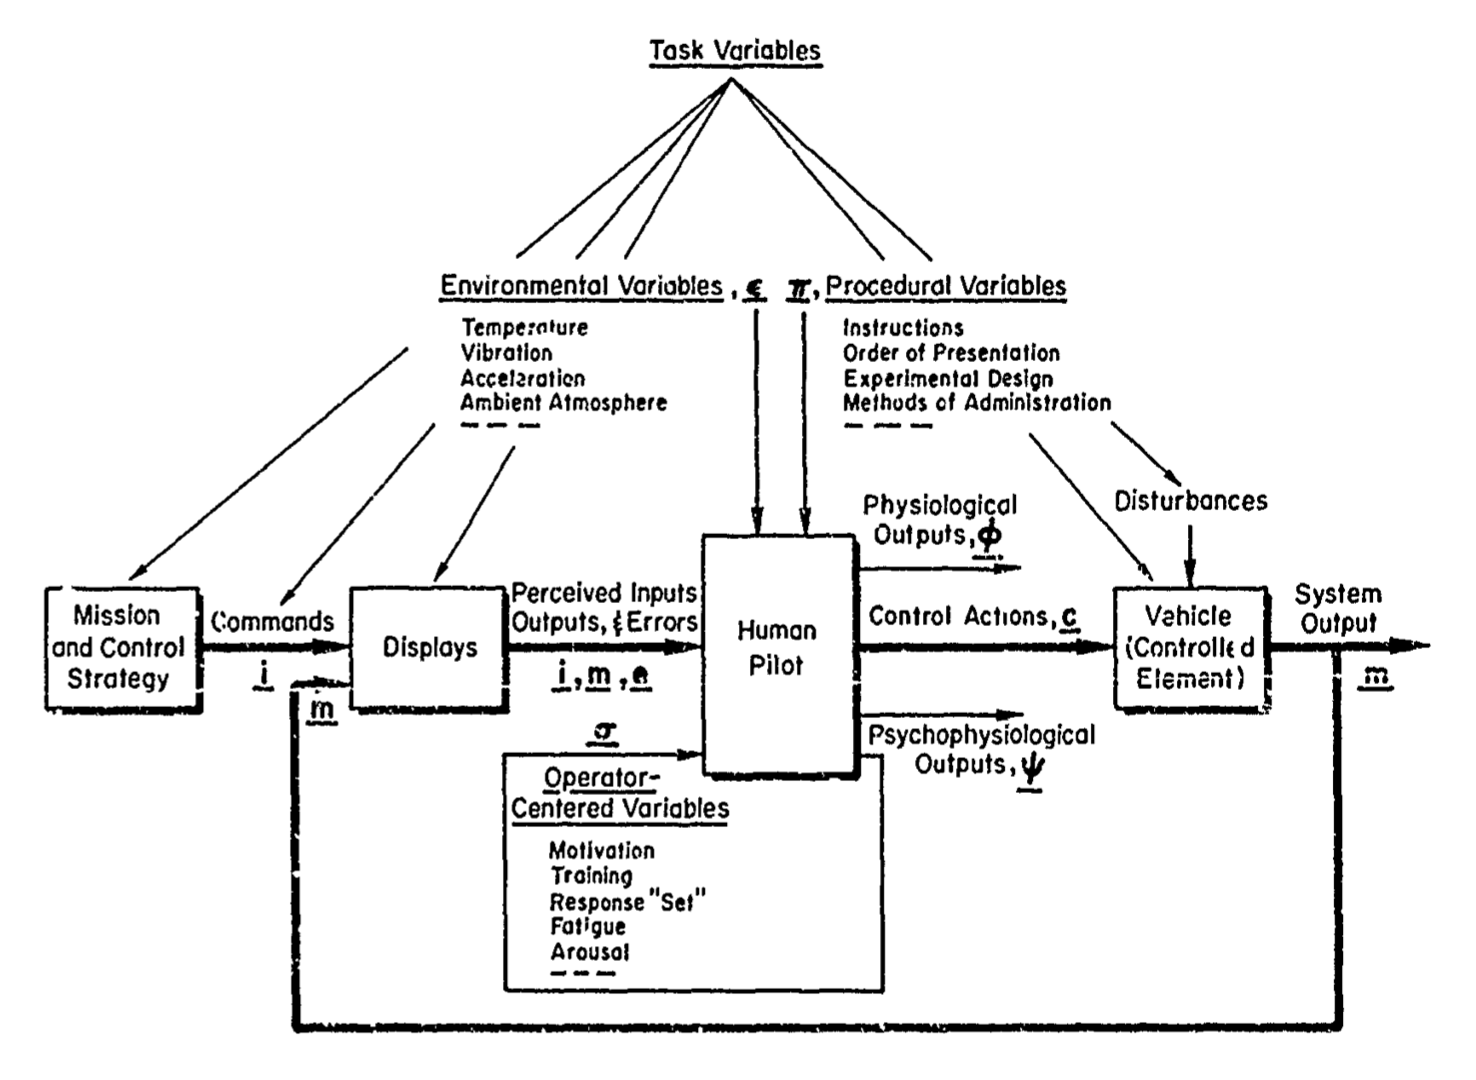
\includegraphics[width=0.8\linewidth]{figures/Screen_Shot_2018-07-25_at_10_37_08_AM.png}
        \caption{Variables affecting the pilot/vehicle system, from~\citep{mcruer_mathematical_1974}.}
        \label{figure:mcruer1974}
    \end{center}
\end{figure}

In addition to popularizing the concept of feedback, the creation of control theory in the early 1940s also provided the tools required for the mathematical modeling of the human pilot.
At the time, new weapons were being created for World War 2 which could only be used effectively with trained operators working in tandem with the machine.
While it was thought that a human could be viewed as a unique kind of servomechanism in the control feedback loop, it was still unclear what factors affected human performance.
Early work by Tustin and others extended the control theory framework and applied these theories to actual human operators~\citep{tustin_investigation_nodate}.
Particular interest was focused on ``attempt[ing] to find the laws of relationship of movement and error. In particular, it was hoped that this relationship [would] be approximately linear and so permit well developed theory of `linear servomechanisms' to be applied to manual control in the same way as it applies to automatic following~\citep{tustin_investigation_nodate}.''
This would allow for the prediction of human performance and the ability to predict the limits of human control.

These early works were summarized in McRuer's 1957 report, ``Dynamic Response of Human Operators''~\citep{mcruer_dynamic_1957}.
This work evaluated measurements for single-input/single-output (SISO) manual control systems and developed predictive models consistent with this data.
Indeed, McRuer writes, ``[i]t is possible, without doing violence to the data, to obtain describing functions which are generally applicable to the results of the many diverse experiments~\citep{mcruer_dynamic_1957}.''
The report concludes by describing a hypothetical transfer function of the human operator which includes a time delay, a neuromuscular lag, and a gain.
McRuer's early model of the complete pilot/vehicle system is presented in Figure~\ref{figure:mcruer1974}.
McRuer revisited these results in 1974, after three decades of supporting engineering and experimental psychology experiments and was able to further generalize these results to a wide variety of system dynamics~\citep{mcruer_mathematical_1974}.
In his study, McRuer completed a detailed analysis which included the human response to proportional, rate/velocity, and acceleration type controlled element dynamics, see Table~\ref{table:mcruer1974a}.
The result of this report was the now famous ``crossover model,'' which relates the operator and controlled element transfer characteristics by the equation
\begin{align}
    Y_c(jw) Y_p(jw) = \dfrac{w_c e^{-jw \tau_e}}{jw}
\end{align}
where $Y_c$ is the controlled element transfer function, $Y_p$ is the approximate human operator transfer function, $w_c$ is the crossover frequency, and $\tau_e$ is the effective time delay of the pilot.
The crossover model is so named as it allows for linear behavior at approximately -20 dB/decade slope in the region of the crossover frequency.
The approximate human operator response to several controlled element transfer functions and their combined open-loop transfer function are presented in Table~\ref{table:mcruer1974b}.
Modeling the human pilot with the crossover enabled a more complete view of the complete pilot/vehicle system, and allowed for human factors recommendations towards the design of new vehicles.
Even today, the crossover model is used as the standard for describing pilot/vehicle systems at the crossover frequency~\citep{mcruer_human_1965, mcruer_mathematical_1974, xu_review_2017}.

\begin{table}[tb]
    \centering
    \caption{Example Applications of Idealized Controlled Element Forms, adapted from~\citep{mcruer_mathematical_1974}}
    \label{table:mcruer1974a}
    \small
    \begin{tabular}{p{.2\linewidth} *{2}{p{.3\linewidth}}}
        \toprule
        Controlled Element Form & Aerospace Control                                & Automobile Control                        \\
        \midrule
        $K_c$                   & Attitude control with ACAH system                & Speed control                             \\
        $\dfrac{K_c}{s}$        & Attitude control with a rate command system      & Heading control at low to moderate speeds \\
        $\dfrac{K_c}{s^2}$      & Attitude control of a spacecraft with damper off & Longitudinal position control             \\
        \bottomrule
    \end{tabular}
\end{table}

\begin{table}[tb]
    \renewcommand{\arraystretch}{2}
    \centering
    \caption{Summary of Human Operator Approximate Characteristics, adapted from~\citep{mcruer_mathematical_1974}}
    \label{table:mcruer1974b}
    \small
    \begin{tabular}{*{3}{c}}
        \toprule
        \thead{Controlled Element                                                            \\ Transfer Function\\ $Y_c$} & \thead{Approximate Human Operator\\ Transfer Function\\ $Y_p$} & \thead{Open-Loop\\ Transfer Function\\ $Y_c Y_p$} \\
        \midrule
        $K_c$              & $\dfrac{K_p e^{-\tau_1 s}}{s}$ & $\dfrac{w_c e^{-\tau_e s}}{s}$ \\
        $\dfrac{K_c}{s}$   & $K_p e^{-\tau_2 s}$            & $\dfrac{w_c e^{-\tau_e s}}{s}$ \\
        $\dfrac{K_c}{s^2}$ & $K_p s e^{-\tau_3 s}$          & $\dfrac{w_c e^{-\tau_e s}}{s}$ \\
        \bottomrule
    \end{tabular}
\end{table}

The continued demand for human pilot models for use in informing vehicle design, as well predicting, preventing, and explaining accidents has led to a variety of more complex pilot models since the creation of the crossover model.
A recent review by Xu et al. in 2017 surveyed the state of the art in human pilot modeling and grouped existing models into three classes of models based on: control theory, human physiology, and intelligence techniques~\citep{xu_review_2017}.
Classical models based on control theory include the McRuer crossover model and optimal control models by Kleinman et al. developed in the early 1970s~\citep{kleinman_optimal_1970, baron_optimal_1970}.
Of these three overarching sets of models, the models based on human physiology are of the greatest interest here.
Models based on human physiology were developed to understand human pilot perception and control behavior, and include the Hess structural model~\citep{hess_structural_1980, hess_model_1990, hess_unified_1997}, Hosman's descriptive model~\citep{hosman_pilots_nodate, hosman_pilots_1999}, and the biodynamic model~\citep{griffin_validation_2001}.
Recent intelligence models take advantage of techniques including fuzzy control and neural networks~\citep{zaychik_conspectus_2006, gestwa_modelling_2003}.

\begin{figure}[tb!]
    \begin{center}
        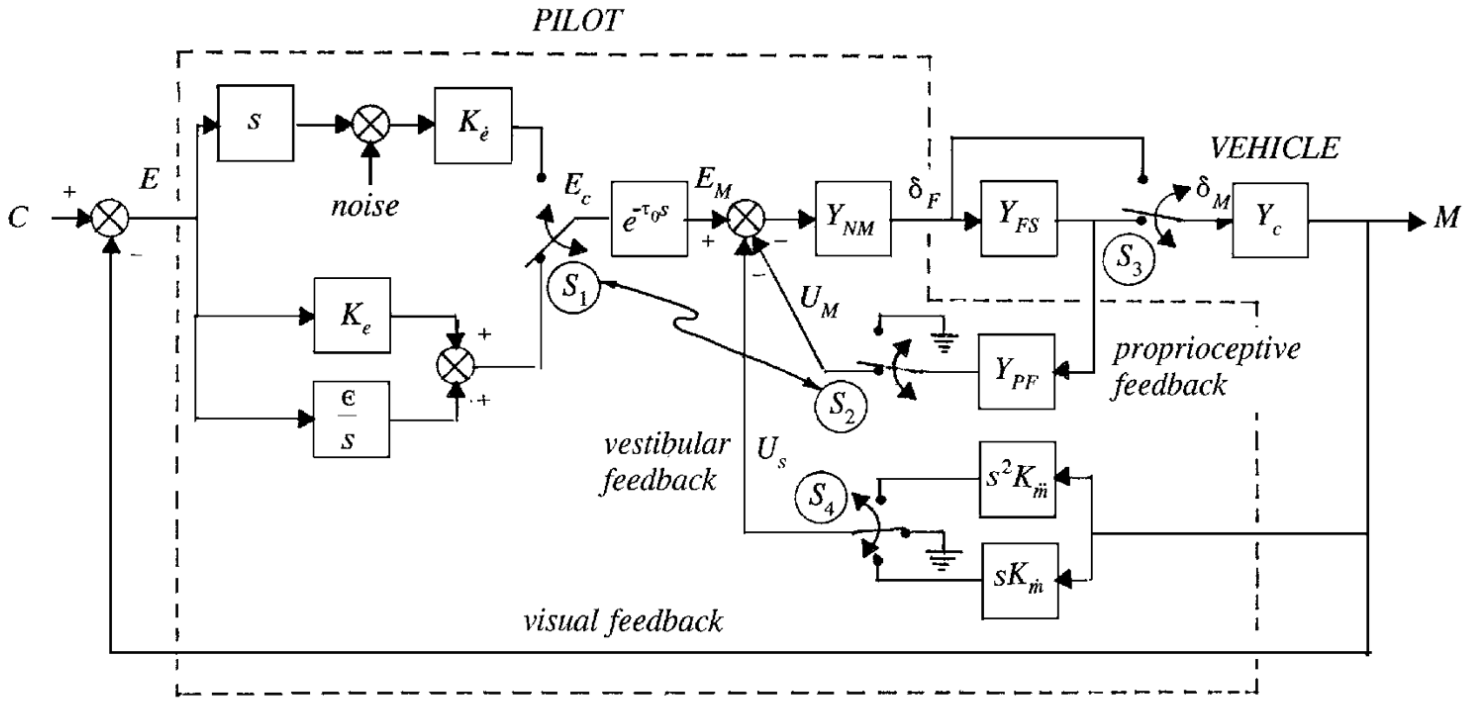
\includegraphics[width=0.8\linewidth]{figures/Screen_Shot_2018-07-31_at_11_21_44_AM.png}
        \caption{The Hess Structural Model of the Human Pilot, from~\citep{hess_unified_1997}.}
        \label{figure:structuralmodel}
    \end{center}
\end{figure}

While the McRuer was very successful in predicting pilot behavior, it it did not attempt ``to describe the underlying structure which contributes to human pilot dynamics~\citep{hess_structural_1980}.''
For this reason, the Hess Structural Model is of particular interest due to the incorporation of multiple sensory channels and models of visual acuity and the time-varying human pilot~\citep{hess_modeling_2009}.
The Structural Model includes the effects of the neuromuscular system, the force-feel characteristics of the input device, and the contributions of proprioceptive, vestibular, and visual feedback, see Figure~\ref{figure:structuralmodel}.
One of the key strengths of the Structural Model is the relatively few number of free parameters that need to be set to predict pilot performance.
The model has been used in predicting and evaluating handling qualities and pilot-induced oscillation rating levels for helicopters, Boeing 747, Lockheed C-5A, and twin ducted-fan aircraft~\citep{hess_analytical_2013, andreea-irina_prediction_2014, grant_handling_2015}.
Hess has also investigated how pilot control characteristics change with time due to flight anomalies, changing flight dynamics, and sudden increases in task demand~\citep{hess_modeling_2009, hess_modeling_2016}.
The results of this model have been compared to the results of a human-in-the-loop simulation for a well trained subject, and showed good comparison~\citep{hess_modeling_2016}.
Recent work from Bachelder et al. has included modifications to the Structural Model to link pilot performance and workload and to enable the modeling of pulsive pilot behavior~\citep{bachelder_modeling_2017, bachelder_linking_2018}.

\section{Research Questions}
\label{sec:intro_questions}
We are interested in measuring, modeling, and predicting the effects of concurrent bandwidth feedback (CBF) on human performance in robotics manual control tasks.
To this end, this proposed research includes three research aims.
These aims build on each other, starting with a compensatory tracking task, extending to a robotics task, and finishing with a descriptive model describing both.
The first aim is complete, and the second and third aims are in progress.
\begin{description}[align=left]
    \item [Aim One] Investigate the effects of concurrent bandwidth feedback on human performance and workload effects in a three-axis manual tracking task.
    \item [Aim Two] Investigate the effects of concurrent bandwidth feedback on human performance and workload effects in a robotics track and capture task.
    \item [Aim Three] Extend the Hess Structural Model of the human pilot to include the effects of concurrent bandwidth feedback.
\end{description}

There are a number of research questions that we intend to answer by completing these aims, which include:
\begin{enumerate}
    \item Can concurrent bandwidth feedback improve human performance in a three-axis manual tracking task?
          \begin{enumerate}
              \item Do 3D augmented reality displays show improved performance compared to traditional 2D displays?
              \item Can performance be increased without increasing workload?
          \end{enumerate}
    \item Can concurrent bandwidth feedback improve performance of simulated robotics tasks?
          \begin{enumerate}
              \item Can CBF reduce the required training time to peak performance?
              \item Can CBF be removed after reaching peak performance without reducing subject performance?
              \item Can performance be increased without increasing workload?
          \end{enumerate}
    \item Can we develop a descriptive model of human performance which includes the effects of concurrent bandwidth feedback?
          \begin{enumerate}
              \item Can we use this model to estimate operational limits?
          \end{enumerate}
\end{enumerate}

\section{Summary}
TODO
